\documentclass[bigger]{beamer}
\usepackage[utf8]{inputenc}
\usepackage[T1]{fontenc}
\usepackage{color}
\usepackage{graphicx}
\usepackage{eurosym}
\usepackage{parcolumns}

\DeclareGraphicsExtensions{.png,.pdf,.jpg}
\graphicspath{{./pics/}}

%Global Background must be put in preamble
\usebackgroundtemplate%
{%
    
\includegraphics[width=\paperwidth,height=\paperheight]{Design.jpg}%
}


\newcommand{\topic}[1]{{\huge{\textcolor{white}{\textbf{#1}}}}}
%\newcommand{\topic}[1]{\textbf{#1}}

\begin{document}
{
\usebackgroundtemplate{
\includegraphics[width=\paperwidth]{Back.jpg}}%
\begin{frame}
%Title: leer, vielleicht noch unsere Namen einfügen
\begin{figure}[H]
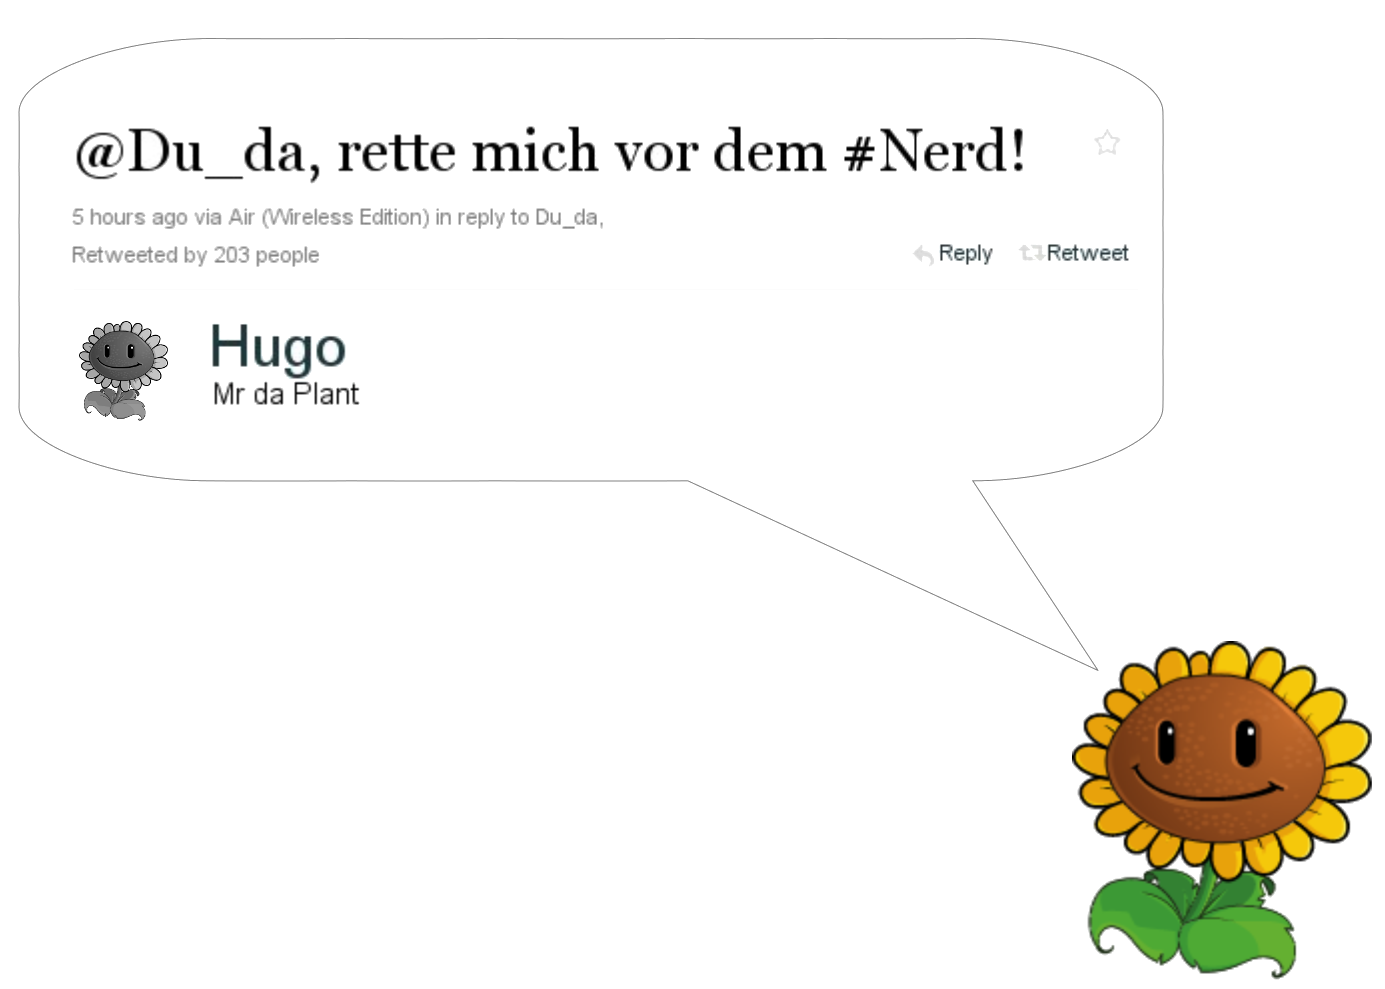
\includegraphics[width=350px]{SprechblaseOR.png}
\end{figure}

\end{frame}
}

\begin{frame}{\topic{Plant Guard}}
   \begin{itemize}
      \item Twitter für Kommunikation
      \item Messungen: Feuchtigkeit*, Temperatur, Wasserstand, uvm.
      \item kann Pflanzen gießen
      \item Erweiterbarkeit gegeben*
      \item Kosten sind relativ gering*
   \end{itemize}
*dazu später mehr Informationen
\end{frame}

\begin{frame}{\topic{Vergleich (andere Projekte)}}
	\begin{itemize}
		\item twittern oder nutzen spezielle Netzwerkprogramme
		\item meist keine Bewässerung (nur bei Hobbyprojekten)
		\item weniger Sensoren (meist nur Feuchtigkeit)
		\item dafür ein Projekt mit Pflanzen-DB für Konfiguration
		\item ein Bausatz/Gerät meist um {100\euro} oder nicht erhältlich
	\end{itemize}
\end{frame}

\begin{frame}{\topic{Vorteile}}
	\begin{itemize}
		\item Pflanzeninfos weltweit verfügbar
		\item Multiuser (z.B. für die Gießvertretung)
		\item automatische Bewässerung
		\item erweiterbar (mehr Sensoren, mehr Pflanzen, ...)
		\item bei Stromausfall wird inzwischen später gegossen
	\end{itemize}
\end{frame}

\begin{frame}{\topic{Probleme}}
	\begin{itemize}
		\item Inkontinenz beim Start, da der Arduino beim Start einige Leitungen auf 1 zieht
		\item wenn PG zuviel gießt, könnte es überlaufen
		\item ziemlich großer Behälter, schlecht zu verstecken, leicht zu kippen
		\item Flasche nur mit Silikon 100\% dicht
		\item viele Kabel, lange Kabel
		\item hohe Kosten bei verteilt stehenden Pflanzen
		\item Behälter muss auch weiterhin höher als die Pflanze stehen
	\end{itemize}
\end{frame}

\begin{frame}{\topic{Kosten}}
	\begin{itemize}
		\item Arduino+WiFly: 60\euro
		\item NetIO+Upgrade: 25\euro
		\item Ventil: 7,50\euro / Pumpe: 13\euro
		\item Sensoren: je nach Anzahl/Art
		\item Platine und Material: wenige\euro
	\end{itemize}
	Summe: ca. 35\euro  bis 75\euro  +x
\end{frame}

\begin{frame}{\topic{Sensoren}}
	\begin{itemize}
		\item Temperatur
		\item Feuchtigkeit
		\item Wasserstand
	\end{itemize}
weitere Ideen folgen
\end{frame}

\begin{frame}{\topic{Temperatur}}
	\begin{itemize}
		\item benötigt einen OpAmp, zweiter ist noch frei
		\item lange Drähte für freie Positionierung
		\item misst im Bereich der Raumtemperatur
		\item direkt auf der Platine
	\end{itemize}
\end{frame}

\begin{frame}{\topic{Feuchtigkeit}}
	\begin{itemize}
		\item zwei lange Metallstäbe, die mit festem Abstand zueinander in den Boden gesteckt werden
		\item statt Widerstand messen wir Kapazität
		\item Nutzung von Wechselstrom (durch Umpolen von 2 Pins)
		\item je niedriger desto feuchter
	\end{itemize}
\end{frame}

\begin{frame}{\topic{Wasserstand}}
	\begin{itemize}
		\item zwei sehr lange Drähte mit festem Abstand
		\item am Arduino werden 4,5 bis 4,9 Volt gemessen
		\item ca. 82stufige Messungen
		\item bedingt wichtig für Nachrichten
		\item sehr wichtig für Pumpen (nur im Wasser betreiben!)
	\end{itemize}
\end{frame}

\begin{frame}{\topic{Aktuatoren/Ventil}}
	\begin{itemize}
		\item leise
		\item nutzt Schwerkraft
		\item z.Z. auf Flaschen-Tank begrenzt
		\item man muss das Ventil richtig ausrichten (um nicht den Bereich um die Pflanze zu gießen)
	\end{itemize}
\end{frame}


\begin{frame}{\topic{mögliche Upgrades}}
	\begin{itemize}
		\item Pumpe statt Ventil (+{5\euro}, mehr Strom nötig, lauter?)
		\item mehr Pflanzen
		\item mehr Sensoren
		\item drahtlose Verbindung
		\item weg vom Arduino/WiFly
		\item DB für Gießparameter
		\item Hardwareverbesserungen
	\end{itemize}
\end{frame}

\begin{frame}{\topic{Pumpe}}
	\begin{itemize}
		\item Ventilansteuerung kompatibel mit einigen Pumpen
		\item Zeiten müssten angepasst werden
		\item Füllstand wäre noch wichtiger
		\item Behälter wäre beliebig, leichter zu verstecken
		\item kein Leck abzudichten
	\end{itemize}
\end{frame}

\begin{frame}{\topic{mehr Pflanzen}}
	\begin{itemize}
		\item drückt die Kosten
		\item spart Strom (gegenüber 1 Arduino pro Pflanze)
		\item mehr Anschlüsse nötig
		\item DeMux: lange Kabel
		\item Funkchip: Protokoll ausarbeiten
	\end{itemize}
\end{frame}

\begin{frame}{\topic{weitere/andere Sensoren}}
	\begin{itemize}
		\item mehrere Feuchtigkeitssensoren
		\item längere Feuchtigkeitssensoren
		\item andere Füllstandssensorik
		\item mehrere Temperatursensoren
		\item +Mikrofon
		\item +Farbsensor
		\item +Barometer
		\item +Kippsensor
	\end{itemize}
\end{frame}

\begin{frame}{\topic{drahtlose Verbindung}}
	\begin{itemize}
		\item man spart sich eine (De)Mux-Platine für mehrere Messstationen
		\item man kann durch Anpassungen am Protokoll mehr Pflanzen versorgen
		\item muss gesichert werden (Übertragungsfehler, ...)
		\item keine Kabel quer durch den Raum/die Etage nötig
	\end{itemize}
\end{frame}

\begin{frame}{\topic{ohne Arduino}}
	\begin{itemize}
		\item NetIO mit Ethersex + SD-Karte = Webserver
		\item geringere Kosten
		\item lange erprobt, sehr ausfallfrei
		\item sicher, da kein WLan benötigt wird
		\item kompatibel mit einem Sender-Chip
	\end{itemize}
\end{frame}

\begin{frame}{\topic{Hardware}}
	\begin{itemize}
		\item Hülle
		\item professionelle Platine
		\item Vorgeben zweier (De)mux-Schaltung (Norm für die Software)
	\end{itemize}
\end{frame}

\begin{frame}{\topic{DB mit Pflanzendaten}}
	\begin{itemize}
		\item man müsste den PG nicht anlernen
		\item dafür aber eine Datenbank mit Informationen füllen und pflegen
		\item ein Dateiformat wird benötigt
		\item eine Uploadfunktion braucht man auch
		\item der User könnte die falsche Pflanze wählen oder in der Größe irren
	\end{itemize}
\end{frame}

\begin{frame}{\topic{Software}}
	\begin{itemize}
		\item 20kb groß (viel für Twitter)
		\item Regelschleife (wenn zu trocken, gieße)
		\item Zeitsteuerung mit Gieße alle ... eine gewisse Menge möglich
		\item liegt unter \url{http://github.com/jasinai/plant\_guard}
	\end{itemize}
\end{frame}



\begin{frame}
%Bild von aktueller Platine
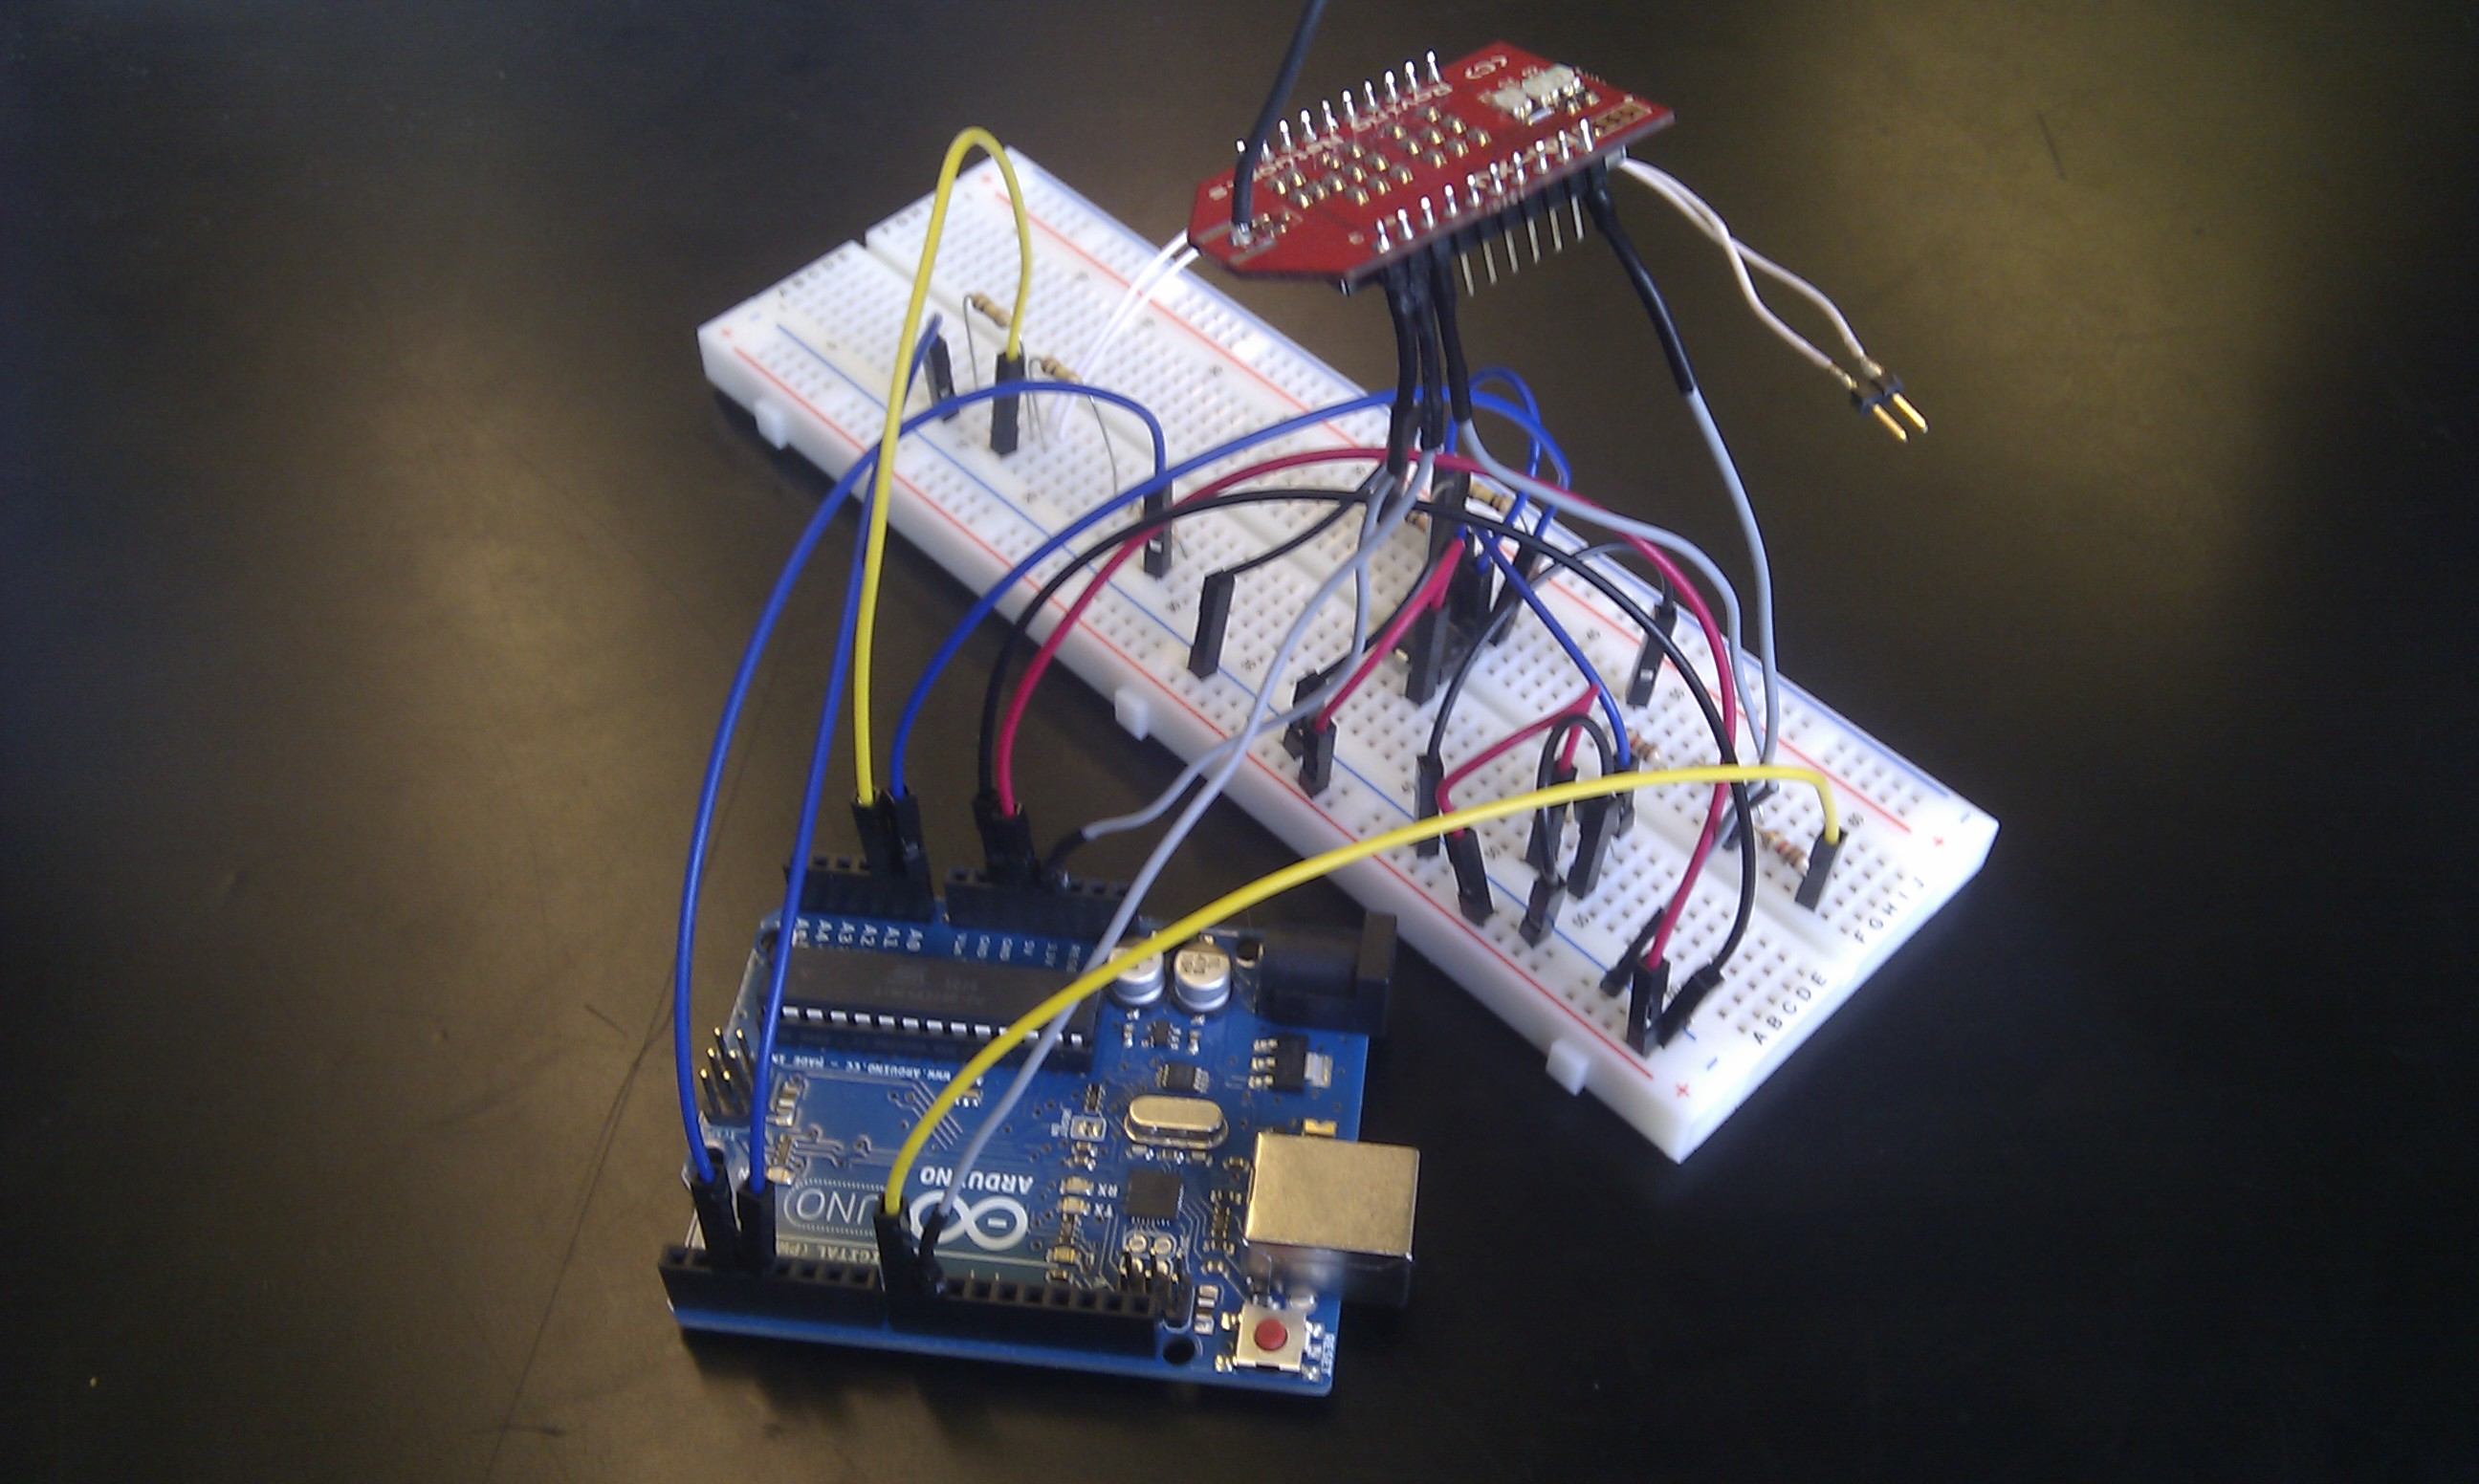
\includegraphics[width=350px]{board.jpg}
\end{frame}
\begin{frame}{\topic{Temperatursensor}}
	\begin{itemize}
		\item LM35 aus dem Starterkit
	\end{itemize}
\end{frame}

\begin{frame}{\topic{Bewässerung}}
%früher / heute vergleich
       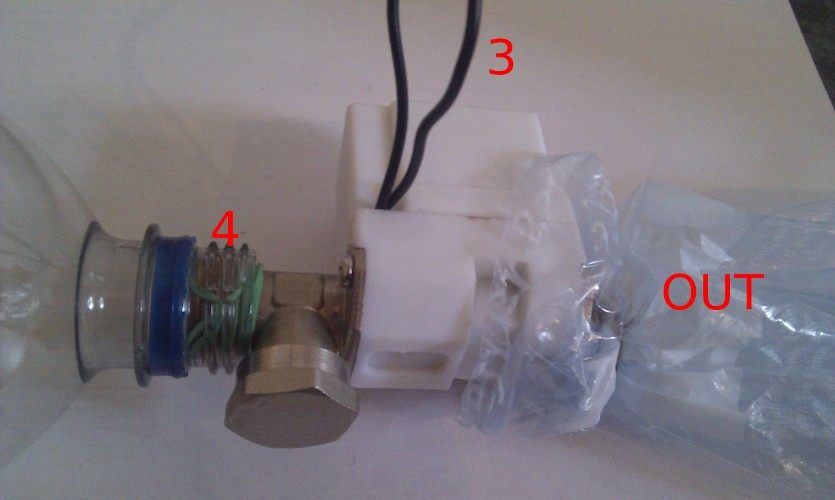
\includegraphics[width=350px]{Anschluss.jpg}
\end{frame}

\begin{frame}{\topic{Bewässerung}}
%früher / heute vergleich
    \begin{columns}
      \column[c]{.50\textwidth}
        \begin{enumerate}
			\item verbreiterte Stellfläche
			\item Messkabel
			\item Ventilansteuerung
			\item Verbindung Vorrat $\rightarrow$ Ventil
        \end{enumerate}
      \column[c]{.50\textwidth}
        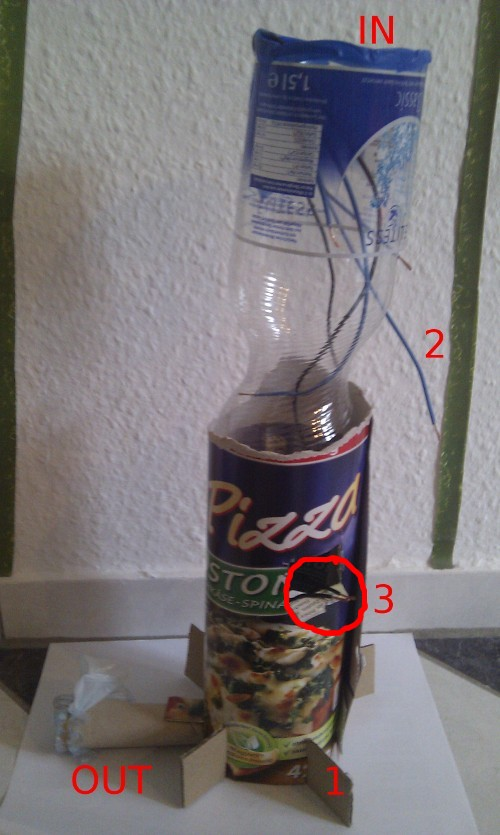
\includegraphics[width=150px]{System.jpg}
    \end{columns}
\end{frame} 

\begin{frame}{\topic{Tweets}}
	\begin{itemize}
		\item "Ich sitze schon x Tage im Dunkeln! Hat da wer die Rollos vergessen?"
		\item "Einen wunderschönen Morgen…" / "Gute Nacht!" (Uhr/Lichtsensor)
		\item "Mir ist langweilig... komm doch mal vorbei und erzähl mir was!” (Zufallsereignis)
		\item "Wasserstand niedrig: Raum x: Pflanzen-ID, Raum y: Hugo, Otto"
		\item "Die Pflanzen Hugo, Otto und Karla wurden erfolgreich gewässert!"
	\end{itemize}
\end{frame}



{
\usebackgroundtemplate{
\includegraphics[width=\paperwidth]{Back.jpg}}%
\begin{frame}{}
	\begin{figure}[H]
		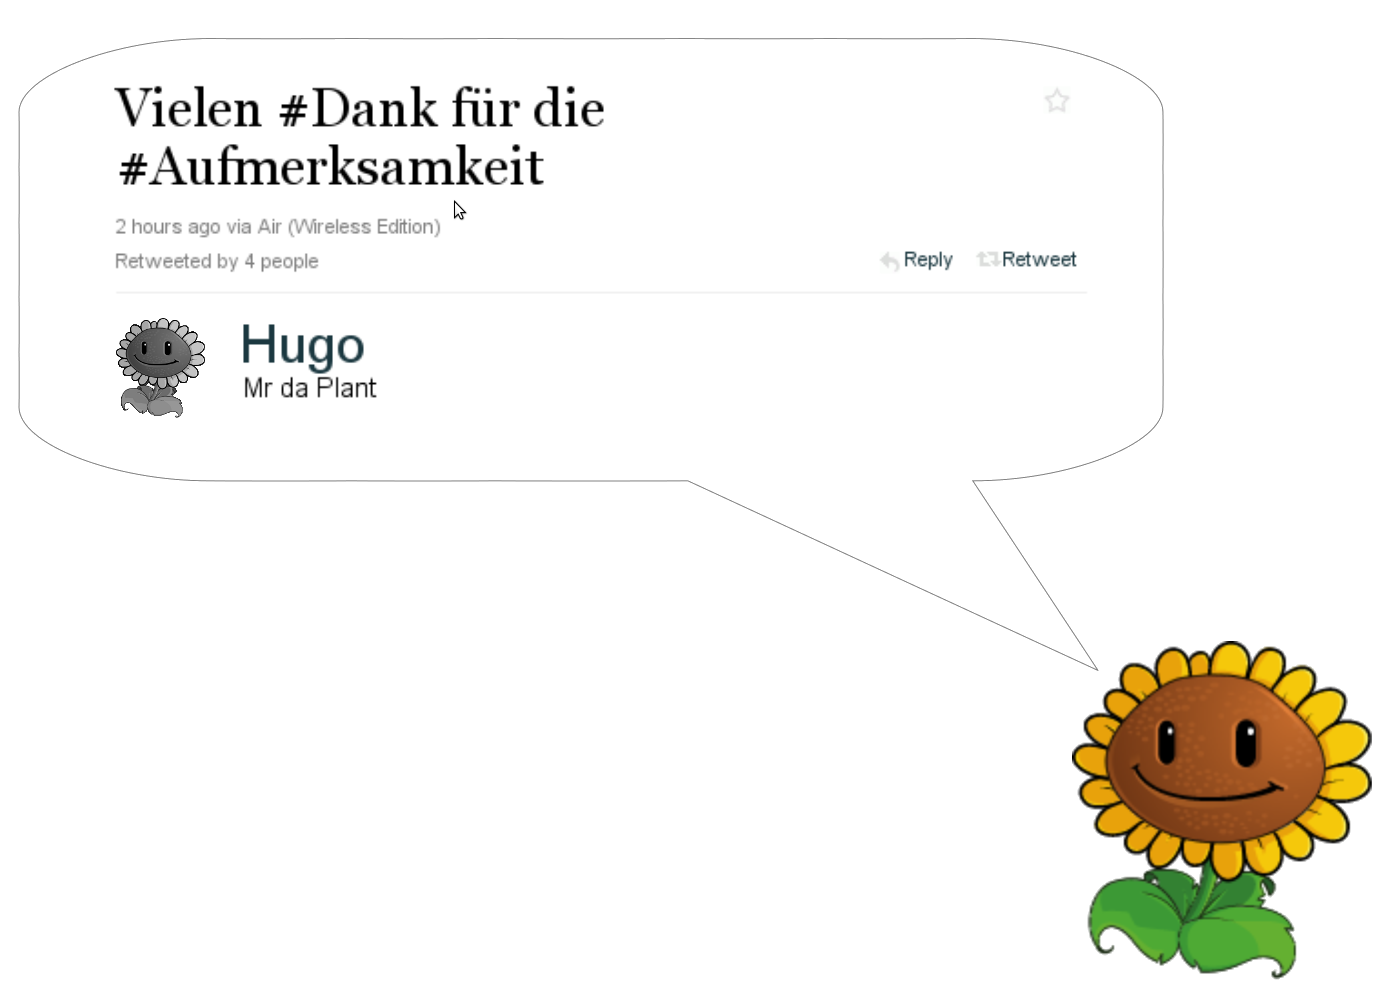
\includegraphics[width=350px]{Danke.png}
	\end{figure}
\end{frame}
}


\end{document}
